
\chapter{A Command Language}

When modelling applications there is often a requirement for some
kind of command language. UML, for example, has state machines where
the actions on the transitions are written in an action language and
describe what happens to the state of the system when the transitions
are fired. One way of providing support for actions in a model is
to allow the user to write commands in their favourite programming
language; the commands are represented in the model as strings. This
is a very weak form of command language, since the strings cannot
be processed easily by the modelling engines. Typically they cannot
be performed at all until the models are exported as program code,
where the command strings are simply embedded in the output. 

More flexibility is provided by modelling the command language. The
model instances can then be interpreted by an engine as part of performing
the overall model. Furthermore, since the commands are modelled, they
can be analysed in various ways and transformed to different target
implementation languages rather than being limited to one.

This chapter is concerned with writing interpreters (translators and
compilers) for a command language. When defining an interpretive semantics
for a language there is often a similar language at hand (at least
the language in which the interpreter is written).There is a choice
choice as to whether the syntax structures are directly interpreted
or whether they are translated to syntax phrases in the existing language.
The advantage of a translational approach is that the execution engine
for the target language already exists and is probably more efficient
than any interpreter we could write for the source language.

Compilers are translators for languages where the target language
is usually highly optimized and very different from the source language.
In principle, however, there is no essential difference between a
translator and a compiler. A language that uses the translational approach
to target a sub-language of itself is often referred to as \emph{desugaring}
the source language.


\section{XCom - A Simple Command Language}

XCom is a simple command language with values that are either records
or are atomic. An atomic data value is a string, integer or boolean.
A record is a collection of named values. XCom is block-structured
where blocks contain type definitions and value definitions. XCom
has simple control structures: conditional statements and loops. The
following is a simple example XCom program that builds a list of even
numbers from 2 to 100:

\begin{lstlisting}
begin
  type Pair is head tail end
  type Nil is end
  value length is 100 end
  value list is new Nil end
  while length > 0 do
    begin
      if length % 2 = 0
      then
        begin
          value pair is new Pair end
          pair.head := length;
          pair.tail := list;
          list := pair;
        end
      end;
      length := length - 1;
    end
end
\end{lstlisting}XCom expressions evaluate to produce XCom values. Values are defined
in the Values package and which is the 
semantic domain for XCom. Values are either atomic: integers and
booleans, or are records. We use a simple representation for records:
a sequence of values indexed by names. XCom records are created by
instantiating XCom record types. A record type is a sequence of names.
Types raise an interesting design issue: should the types be included
as part of the semantic domain since evaluation of certain XCom program
phrases give rise to types that are used later in the execution to
produce records. The answer to the question involves the phase distinction
that occurs between static analysis (or execution)
and dynamic execution. Types are often viewed
as occurring only during static analysis; although this is not always
the case.

We will show how the semantics of XCom can be defined with and without
dynamic types. All XCom values are instances of sub-classes of the class
Value.

\begin{lstlisting}
context Bool
  @Operation binAnd(Bool(b))
    Bool(value and b)
  end
context Bool
  @Operation binOr(Bool(b))
    Bool(value or b)
  end
context Int
  @Operation binAdd(Int(n))
    Int(value + n)
  end
\end{lstlisting}Record types are sequences of names. Records are sequences of values
indexed by names; the names are found by navigating to the

type of the record:

\begin{lstlisting}
context Record
  @Operation lookup(name:String)
    fields->at(type.names->indexOf(name))
  end
context Record
  @Operation update(name:String,value:Element)
    fields->setAt(type.names->indexOf(name),value)
  end
\end{lstlisting}A new record is produced by performing a new
expression. The type to instantiate is given as a string. An alternative
representation for types in new expressions
would be to permit an arbitrary expression that
evaluates to produce a type. This design choice would rule out static
typing and force the language to have dynamic types. We wish to use
XCom to illustrate the difference between dynamic and static types
in semantic definitions so we use strings to name types in 
new expressions:

The concrete syntax of expressions is defined by the XBNF grammar
for the class Exp:

\begin{lstlisting}
@Grammar 
  // Start at Exp. Logical operators bind weakest.
  Exp ::= e = ArithExp [ op = LogicalOp l = Exp { BinExp(op,e,l) } ].
  LogicalOp ::= 'and' { "and" } | 'or' { "or" }.
  // The '.' for field ref binds tighter than '+' etc.
  ArithExp ::= e = FieldRef [ op = ArithOp a = FieldRef { BinExp(op,e,a) } ].
  ArithOp ::= '+' { "+" }.
  // A field reference '.' optionally follows an atomic expression.
  FieldRef ::= e = Atom ('.' n = Name { FieldRef(e,n) } | { e }).
  // Atomic expressions can be arbitrary exps if in ( and ).
  Atom ::= Const | Var | New | '(' Exp ')'.
  Const ::= IntConst | BoolConst.
  IntConst ::= i = Int { Const(i) }.
  BoolConst ::= 'true' { Const(true) } | 'false' { Const(false) }.
  Var ::= n = Name { Var(n) }.
  New ::= 'new' n = Name { New(n) }.
end
\end{lstlisting}
XCom statements are used to:

\begin{itemize}
\item Introduce new names associated with either types or values.
\item Control the flow of execution.
\item Perform side effects on records.
\end{itemize}
A block (as in Pascal or C) contains local definitions. Names introduced
in a block are available for the rest of the statements in the block
(including sub-blocks) but are not available when control exits from
the block. A declaration introduces either a type or a value binding.
A type declaration associates a type name with a sequence of field
names. To keep things simple we don't associate fields with types.
A value declaration associates a name with a new value. The value
is produced by performing an expression at run-time. A while statement
involves a test and a body. An if statement involves a test, a then-part
and an else-part:

\begin{lstlisting}
@Grammar extends Exp.grammar
  Statement ::= 
    Block 
  | Declaration 
  | While 
  | If 
  | Update 
  | FieldUpdate.
  Block ::= 'begin' s = Statement* 'end' { Block(s) }.
  Declaration ::= 
    TypeDeclaration 
  | ValueDeclaration.
  TypeDeclaration ::= 
    'type' n = Name 'is' ns = Name* 'end' 
    { TypeDeclaration(n,ns) }.
  ValueDeclaration ::= 
    'value' n = Name 'is' e = Exp 'end' 
    { ValueDeclaration(n,e) }.
  FieldUpdate ::= 
    e = Exp '.' n = Name ':=' v = Exp ';' 
    { FieldUpdate(e,n,v) }.
  While ::= 
    'while' e = Exp 'do' s = Statement 'end' 
    { While(e,s) }.
  If ::= 
    'if' e = Exp 
    'then' s1 = Statement 
    'else' s2 = Statement 
    'end' 
    { If(e,s1,s2) }.
  Update ::= 
    n = Name ':=' e = Exp ';' 
    { Update(n,e) }.
end
\end{lstlisting}
\section{An Evaluator for XCom}

As described in the introduction we are interested in defining XCom
operational semantics. We will do this in a number of different ways
in the rest of this note. The first, and possibly most straightforward,
approach is to define an interpreter for XCom
in the XOCL language. This involves writing an 
eval operation for each of the XCom syntax classes. The 
eval operation must be parameterized with respect to any context
information that is required to perform the evaluation. An XCom program
p is then evaluated in a context 
e by: p.eval(e).


\subsection{Evaluating Expressions}

Expression evaluation is defined by adding eval operations to each
class. This section defines the eval operation:

\begin{lstlisting}
context Const
  @Operation eval(env)
    @TypeCase(value)
      Boolean do Bool(value) end
      Integer do Int(value) end
    end
  end
\end{lstlisting}Evaluation of a variable involves looking up the current value. The
value is found in the current context of evaluation: this must contain
associations between variable names and their values:

\begin{lstlisting}
context Var
  @Operation eval(env)
    env.lookup(name)
  end
\end{lstlisting}Evaluation of a binary expression involves evaluation of the sub-expressions
and then selecting an operation based on the operation name. The following
shows how XCom semantics is completely based on XOCL semantics since
+ in XCom is performed by + in XOCL:

\begin{lstlisting}
context BinExp
  @Operation eval(env)
    @Case op of
      "and" do left.eval(env).binAnd(right.eval(env)) end
      "or" do left.eval(env).binOr(right.eval(env)) end
      "+" do left.eval(env).binAdd(right.eval(env)) end
    end
  end
\end{lstlisting}Creation of new records is performed by evaluaing a new expression.
The interpreter has dynamic types so the type to instantiate is found
by looking up the type name in the current environment:

\begin{lstlisting}
context New
  @Operation eval(env)
    env.lookup(type).new()
  end
\end{lstlisting}Field reference is defined as follows:

\begin{lstlisting}
context FieldRef
  @Operation eval(env)
    value.eval(env).lookup(name)
  end
\end{lstlisting}
\subsection{Evaluating Statements}

XCom statements are performed in order to introduce new names, control
flow or to update a record field. Statements are defined to evaluate
in a context and must observe the rules of scope that require variables
are local to the block that introduces them. The context of execution
is an environment; evaluation of a statement may update the supplied
environment, so statement evaluation returns an environment:

\begin{lstlisting}
  context ValueDeclaration
    @Operation eval(env)
      env.bind(name,value.eval(env))
    end
\end{lstlisting}A type declaration extends the supplied environment with a new type:

\begin{lstlisting}
context TypeDeclaration
  @Operation eval(env)
    env.bind(name,Type(names))
  end
\end{lstlisting}A block must preserve the supplied environment when its evaluation
is complete. Each statement in the block is performed in turn and
may update the current environment:

\begin{lstlisting}
context Block
  @Operation eval(originalEnv)
    let env = originalEnv
    in @For statement in statements do
         env := statement.eval(env)
       end
    end;
    originalEnv
  end
\end{lstlisting}A while statement continually performs the body while the test expression
returns true. A while body is equivalent to a block; so any updates
to the supplied environment that are performed by the while body are
discarded on exit:

\begin{lstlisting}
context While
  @Operation eval(originalEnv)
    let env = orginalEnv
    in @While test.eval(env).value do
         env := body.eval(env)
       end;
       originalEnv
    end
  end
\end{lstlisting}An if statement conditionally performs one of its sub-statements:

\begin{lstlisting}
context If
  @Operation eval(env)
    if test.eval(env).value
    then thenPart.eval(env)
    else elsePart.eval(env)
    end
  end
\end{lstlisting}\begin{lstlisting}
context FieldUpdate
  @Operation eval(env)
    record.eval(env).update(name,value.eval(env))
  end
context Update
  @Operation eval(env)
    env.update(name,value.eval(env))
  end
\end{lstlisting}
\section{A Translator for XCom with Run-Time Types}

The previous section defines an interpreter for XCom. This is an appealing
way to define the operational semantics of a language because the
rules of evaluation work directly on the abstract syntax structures.
However the resulting interpreter can often be very inefficient. Furthermore,
an interpreter can lead to an \emph{evaluation phase distinction}.

Suppose that XCom is to be embedded in XOCL. XOCL has its own interpretive
mechanism (the XMF VM); at the boundary between XOCL and XCom the
XOCL interpretive mechanism must hand over to the XCom interpreter
-- the XCom code that is performed is a data structure, a completely
alien format to the VM. This phase distinction can lead to problems
when using standard tools, such as save and load mechanisms, with
respect to the new language. For example a mechanism that can save
XOCL code to disk cannot be used to save XCom code to disk (it can,
however, be used to save the XCom interpreter to disk).

An alternative strategy is to translate the source code of XCom to
a language for which we have an efficient implementation. No new interpretive
mechanism is required and no phase distinction arises. Translation
provides the opportunity for static analysis (since translation is
performed prior to executing the program). As we mentioned earlier,
static analysis can translate out any type information from XCom programs;
the resulting program does not require run-time types.

Since static analysis requires a little more work, this section describes
a simple translation from XCom to XOCL that results in run-time types;
the subsequent section showshow this can be extended to analyse types
statically and remove them from the semantic domain.


\subsection{Translating Expressions}

Translation is defined by adding a new operation desugar\} to each
sbatract syntax class. There is no static analysis, so the operation
does not require any arguments. The result of the operation is a value
of type Performable which is the type of elements that can be executed
by the XMF execution engine. An XCom constant is translated to an
XOCL constant:

\begin{lstlisting}
context Const
  @Operation desugar1():Performable
    value.lift()
  end
\end{lstlisting}An XCom binary expression is translated to an XOCL binary expression.
Note that the sub-expressions are also translated:

\begin{lstlisting}
context BinExp
  @Operation desugar1():Performable
    @Case op of
      "and" do [| <left.desugar1()> and <right.desugar1()> |] end
      "or" do [| <left.desugar1()> and <right.desugar1()> |] end
      "+" do [| <left.desugar1()> + <right.desugar1()> |] end
    end
  end
\end{lstlisting}An XCom new expression involves a type name. Types will be bound to
the appropriate variable name in the resulting XOCL program; so the
result of translation is just a message new sent to the value of the
variable whose name is the type name:

\begin{lstlisting}
context New
  @Operation desugar1():Performable
    [| <OCL::Var(type)>.new() |]
  end
\end{lstlisting}XCom variables are translated to XOCL variables:

\begin{lstlisting}
context Var
  @Operation desugar1():Performable
    OCL::Var(name)
  end
\end{lstlisting}XCom field references are translated to the appropriate call on a
record:

\begin{lstlisting}
context FieldRef
  @Operation desugar1():Performable
    [| <value.desugar1()>.ref(<StrExp(name)>) |]
  end
\end{lstlisting}
\subsection{Translating Statements}

An XCom statement can involve local blocks. The equivalent XOCL expression
that provides local definitions is let. A let expression consists
of a name, a value expression and a body expression. Thus, in order
to translate an XCom declaration to an XOCL let we need to be passed
the body of the let. This leads to a translational style for XCom
commands called \emph{continuation passing} where each desugar1 operation
is supplied with the XOCL command that will be performed next.

A type declaration is translated to a local definition for the type
name. Note that the expression names.lift() translates the sequence
of names to an expression that, when performed, produces the same
sequence of names: list is a means of performing evaluation in reverse:

\begin{lstlisting}
context TypeDeclaration
  @Operation desugar1(next:Performable):Performable
    [| let <name> = Type(<names.lift()>) 
       in <next> 
       end |]
  end
\end{lstlisting}A value declaration is translated to a local decinition:

\begin{lstlisting}
context ValueDeclaration
  @Operation desugar1(next:Performable):Performable
    [| let <name> = <value.desugar1()> 
       in <next> 
       end |]
  end
\end{lstlisting}A block requires each sub-statement to be translated in turn. Continuation
passing allows us to chain together the sequence of statements and
nest the local definitions appropriately. The following auxiliary
operation is used to implement block-translation:

\begin{lstlisting}
context Statements
  @Operation desugar1(statements,next:Performable):Performable
    @Case statements of
      Seq{} do 
        next 
      end
      Seq{statement | statements} do 
        statement.desugar1(desugar1(statements,next)) 
      end
    end
  end
\end{lstlisting}Translation of a block requires that the XOCL local definitions are
kept local. Therefore, the sub-statements are translated by chaining
them together and with a final continuation of null. Placing the result
in sequence with next ensures that any definitions
are local to the block.

\begin{lstlisting}
context Block
  @Operation desugar1(next:Performable):Performable
    [| <desugar1(statements,[| null |])> ; 
    <next> |]
end
\end{lstlisting}A while statement is translated to the equivalent expression in XOCL:

\begin{lstlisting}
context While
  @Operation desugar1(next:Performable):Performable
    [| @While <test.desugar1()>.value do
         <body.desugar1([|null|])>
       end;
       <next> |]
end
\end{lstlisting}An if statement is translated to an equivalent expression in XOCL:

\begin{lstlisting}
context If
  @Operation desugar1(next:Performable):Performable
    [| if <test.desugar1()>.value
       then <thenPart.desugar1(next)>
       else <elsePart.desugar1(next)>
       end |]
end
\end{lstlisting}\begin{lstlisting}
context FieldUpdate
@Operation desugar1(next:Performable):Performable
  [| <record.desugar1()>.update(<StrExp(name)>,<value.desugar1()>);
     <next> |]
end
context Update
  @Operation desugar1(next:Performable):Performable
    [| <name> := <value.desugar1()>;
       <next> |]
end
\end{lstlisting}
\section{A Translator for XCom without Run-Time Types}

It is usual for languages to have a static (or \emph{compile time})
phase and a dynamic (or \emph{run time}) phase. Many operational features
of the language can be performed statically. This includes type analysis:
checking that types are defined before they are used and allocating
appropriate structures when instances of types are created. This section
shows how the translator for XCom to XOCL from the previous section
can be modified so that type analysis is performed and so that types
do not occur at run-time.


\subsection{Translating Expressions}

Since types will no longer occur at run-time we will simplify the
semantic domain slightly and represent records as \emph{a-lists}.
An a-list is a sequence of pairs, the first element of each pair is
a key and the second element is a value. In this case a record is
an a-list where the keys are field name strings. XOCL provides operations
defined on sequences that are to be used as a-lists: {\tt l->lookup(key)}
and {\tt l->set(key,value)}.

The context for static analysis is a type environment. Types now occur
at translation time instead of run-time therefore that portion of
the run-time context that would contain associations between type
names and types occurs during translation. Translation of a constant
is as for desugar1. Translation of binary expressions is as for desugar1
except that all translation is performed by desugar2:

\begin{lstlisting}
context BinExp
  @Operation desugar2(typeEnv:Env):Performable
    @Case op of
      "and" do 
        [| <left.desugar2(typeEnv)> and
           <right.desugar2(typeEnv)> |] 
      end
      "or" do 
        [| <left.desugar2(typeEnv)> or 
           <right.desugar2(typeEnv)> |] 
      end 
      "+" do 
        [| <left.desugar2(typeEnv)> + 
           <right.desugar2(typeEnv)> |] end
      end
  end
\end{lstlisting}Translation of a variable is as before. A new expression involves
a reference to a type name. The types occur at translation time and
therefore part of the evaluation of new can occur during translation.
The type should occur in the supplied type environment; the type contains
the sequence of field names. The result of translation is an XOCL
expression that constructs an a-list based on the names of the fields
in the type. The initial value for each field is null:

\begin{lstlisting}
context New
  @Operation desugar2(typeEnv:Env):Performable
    if typeEnv.binds(type)
    then
      let type = typeEnv.lookup(type)
      in type.names->iterate(name exp = [| Seq{} |] | 
          [| <exp>->bind(<StrExp(name)>,null) |])
      end
    else self.error("Unknown type " + type)
    end
  end
\end{lstlisting}A field reference expression is translated to an a-list lookup expression:

\begin{lstlisting}
context FieldRef
  @Operation desugar2(typeEnv:Env):Performable
    [| <value.desugar2(typeEnv)>->lookup(<StrExp(name)>) |] 
  end
\end{lstlisting}
\subsection{Translating Statements}

A statement may contain a local type definition. We have already discussed
continuation passing with respect to desugar1 where the context for
translation includes the next XOCL expression to perform. The desugar2
operation cannot be supplied with the next XOCL expression because
this will depend on whether or not the current statement extends the
type environment. Therefore, in desugar2 the continuation is an operation
that is awaiting a type environment and produces the next XOCL expression.
A type declaration binds the type at translation time and supplies
the extended type environment to the continuation:

\begin{lstlisting}
context TypeDeclaration
  @Operation desugar2(typeEnv:Env,next:Operation):Performable
    next(typeEnv.bind(name,Type(names)))
  end
\end{lstlisting}A value declaration introduces a new local definition; the body is
created by supplying the unchanged type environment to the continuation:

\begin{lstlisting}
context ValueDeclaration
  @Operation desugar2(typeEnv:Env,next:Operation):Performable
    [| let <name> = <value.desugar2(typeEnv)> 
       in <next(typeEnv)> 
       end |]
  end
\end{lstlisting}Translation of a block involves translation of a sequence of sub-statements.
The following auxiliary operation ensures that the continuations are
chained together correctly:

\begin{lstlisting}
context Statements
  @Operation desugar2(statements,typeEnv,next):Performable
    @Case statements of
      Seq{} do 
        next(typeEnv)
      end
      Seq{statement | statements} do 
        statement.desugar2(
          typeEnv,
          @Operation(typeEnv)
            desugar2(statements,typeEnv,next)
          end) 
      end
    end
  end
\end{lstlisting}A block is translated to a sequence of statements where local definitions
are implemented using nested let expressions in XOCL. The locality
of the definitions is maintained by sequencing the block statements
and the continuation expression:

\begin{lstlisting}
context Block
  @Operation desugar2(typeEnv:Env,next:Operation):Performable
    [| <desugar2(
         statements,
         typeEnv,
         @Operation(ignore) 
           [| null |] 
         end)>;
       <next(typeEnv)> |]
  end
\end{lstlisting}A while statement is translated so that the XOCL expression is in
sequence with the expression produced by the contintuation:

\begin{lstlisting}
context While
  @Operation desugar2(typeEnv:Env,next:Operation):Performable
    [| @While <test.desugar2(typeEnv)>.value do
         <body.desugar2(typeEnv,@Operation(typeEnv) [| null |] end)>
       end;
       <next(typeEnv)> |]
  end
\end{lstlisting}The if statement is translated to an equivalent XOCL expression:

\begin{lstlisting}
context If
  @Operation desugar2(typeEnv:Env,next:Operation):Performable
    [| if <test.desugar2(typeEnv)>.value
       then <thenPart.desugar2(typeEnv,next)>
       else <elsePart.desugar2(typeEnv,next)>
       end |]
  end
\end{lstlisting}\begin{lstlisting}
context FieldUpdate
  @Operation desugar2(typeEnv:Env,next:Operation):Performable
    [| <record.desugar2(typeEnv)>.update(
         <StrExp(name)>,
         <value.desugar2(typeEnv)>);
       <next(typeEnv)> |]
  end

context Update
  @Operation desugar2(typeEnv:Env,next:Operation):Performable
    [| <name> := <value.desugar2(typeEnv)>;
       <next(typeEnv)> |]
  end
\end{lstlisting}
\section{Compiling XCom}

The previous section shows how to perform static type anslysis while
translating XCom to XOCL. XOCL is then translated to XMF VM instructions
by the XOCL compiler (another translation process). The result is
that XCom cannot to anything that XOCL cannot do. Whilst this is not
a serious restriction, there may be times where a new language wishes
to translate directly to the XMF VM that XOCL does not support. This
section shows how XCom can be translated directly to XMF VM instructions.


\subsection{Compiling Expressions}

\begin{lstlisting}
context Exp
  @AbstractOp compile(typeEnv:Env,valueEnv:Seq(String)):Seq(Instr)
  end
\end{lstlisting}\begin{lstlisting}
context Const
  @Operation compile(typeEnv,valueEnv)
    @TypeCase(value)
      Boolean do 
        if value 
        then Seq{PushTrue()} 
        else Seq{PushFalse()} 
        end 
      end
      Integer do 
        Seq{PushInteger(value)}
      end
    end
  end
\end{lstlisting}\begin{lstlisting}
context Var
  @Operation compile(typeEnv,valueEnv)
    let index = valueEnv->indexOf(name)
    in if index < 0
       then self.error("Unbound variable " + name)
       else Seq{LocalRef(index)}
       end
    end
  end
\end{lstlisting}\begin{lstlisting}
context BinExp
  @Operation compile(typeEnv,valueEnv):Seq(Instr)
    left.compile(typeEnv,valueEnv) + 
    right.compile(typeEnv,valueEnv) +
    @Case op of
      "and" do Seq{And()} end
      "or" do Seq{Or()} end
      "+" do Seq{Add()} end
    end
  end
\end{lstlisting}\begin{lstlisting}
context New
  @Operation compile(typeEnv,valueEnv):Seq(Instr)
    self.desugar2(typeEnv).compile()
  end
\end{lstlisting}\begin{lstlisting}
context FieldRef
  @Operation compile(typeEnv,valueEnv):Seq(Instr)
    Seq{StartCall(),
        PushStr(name)} +
    value.compile(typeExp,valueExp) +
    Seq{Send("lookup",1)}
  end
\end{lstlisting}
\subsection{Compiling Statements}

\begin{lstlisting}
context Statement
  @AbstractOp compile(typeEnv:Env,varEnv:Seq(String),next:Operation):Seq(Instr)
  end
\end{lstlisting}\begin{lstlisting}
context TypeDeclaration
  @Operation compile(typeEnv,varEnv,next)
    next(typeEnv.bind(name,Type(names)),varEnv)
  end
\end{lstlisting}\begin{lstlisting}
context ValueDeclaration
  @Operation compile(typeEnv,varEnv,next)
    value.compile(typeEnv,varEnv) +
    Seq{SetLocal(name,varEnv->size),
        Pop()} +
    next(typeEnv,varEnv + Seq{name})
  end
\end{lstlisting}\begin{lstlisting}
context Statements
  @Operation compile(statements,typeEnv,varEnv,next)
    @Case statements of
      Seq{} do 
        next(typeEnv,varEnv) 
      end
      Seq{statement | statements} do 
        statement.compile(
          typeEnv,
          varEnv,
          @Operation(typeEnv,varEnv)
            compile(statements,typeEnv,varEnv,next)
          end) 
     end
   end
  end
\end{lstlisting}\begin{lstlisting}
context Block
  @Operation compile(typeEnv,varEnv,next)
    compile(
     statements,
     typeEnv,
     varEnv,
       @Operation(localTypeEnv,localVarEnv) 
         next(typeEnv,varEnv) 
       end)
   end
\end{lstlisting}\begin{lstlisting}
context While
  @Operation compile(typeEnv,varEnv,next)
    Seq{Noop("START")} +
    test.compile(typeEnv,varEnv) +
    Seq{SkipFalse("END")} +
    body.compile(typeEnv,varEnv,
      @Operation(typeEnv,varEnv) 
        Seq{} 
      end) +
    Seq{Skip("START")} +
    Seq{Noop("END")} +
    next(typeEnv,varEnv)
  end
\end{lstlisting}

\section{Flow Graphs}

The previous section has shown how to represent the abstract syntax
of XCom as textual concrete syntax. We would like to compare this
to a graphical concrete syntax for XCom and show how the XCom programs
can be developed graphically rather than textually.

\emph{Flow Graphs} are a standard way of representing imperative programs.
Flow graph nodes are labelled with either program statements or boolean
expressions. Flow graph edges are labelled with next if the edge represents
the control flow between statements, true if the edge represents the
control flow arising when a test succeeds, and false if the edge represents
the flow from a test failure.

%
\begin{figure}
\begin{center}

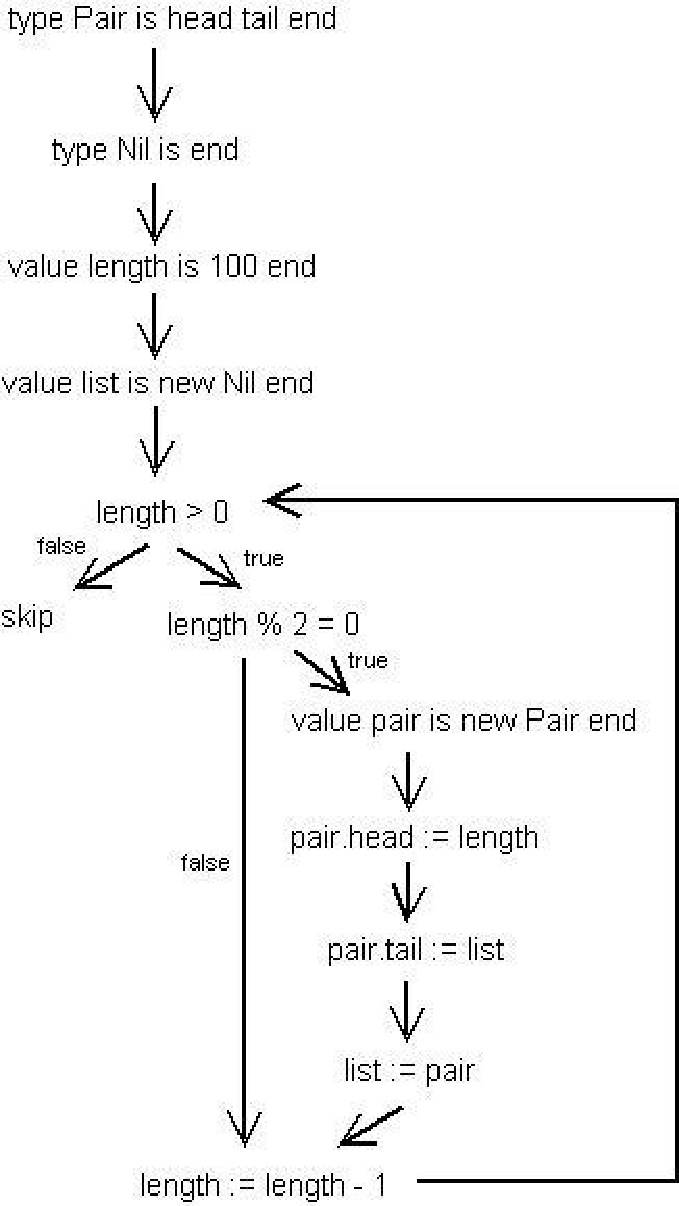
\includegraphics[width=12cm]{LanguageEngineering/Commands/Images/Program}

\caption{\label{fig:An-Example-Flow}An Example Flow Graph}

\end{center}
\end{figure}


Figure \ref{fig:An-Example-Flow}shows an example flow graph corresponding
to the original example XCom program. Note that a while loop is represented
as a test node whose true edge eventually leads back to the test node.
XMF provides a packages called Graph that provides a basic collection
of graph structures and operations. A graph node is created: Node(l)
where l is the label on the graph node. A graph edge is created: 
Edge(l,s,t) where l is the label on the edge,
s is the source node for the edge and 
t is the target node for the edge. A graph is created: 
Graph(N,E) where N is a set of nodes and
E is a set of edges. The graph shown in figure
\ref{fig:An-Example-Flow} is constructed as follows where classes
Node and Edge have been
specialized appropriately:

\begin{lstlisting}
let n1 = Statement("type Pair is head tail end");
n2 = Statement("type Nil is end");
n3 = Statement("value length is 100 end");
n4 = Statement("value list is new Nil end");
n5 = Guard("length > 0");
n6 = Guard("length % 2 = 0");
n7 = Statement("value pair is new Pair end");
n8 = Statement("pair.head := length;");
n9 = Statement("pair.tail := list;");
n10 = Statement("list := pair;");
n11 = Statement("length := length - 1;");
n12 = Statement("skip") then
e1 = Next(n1,n2);
e2 = Next(n2,n3);
e3 = Next(n3,n4);
e4 = Next(n4,n5);
e5 = True(n5,n6);
e6 = True(n6,n7);
e7 = Next(n7,n8);
e8 = Next(n8,n9);
e9 = Next(n9,n10);
e11 = Next(n10,n11);
e12 = Next(n11,n5);
e13 = False(n6,n11);
e14 = False(n5,n12)
in Graph(Set{n1,n2,n3,n4,n5,n6,n7,n8,n9,n10,n11,n12},
Set{e1,e2,e3,e4,e5,e6,e7,e8,e9,10,e11,e12,e13,e14})
end
\end{lstlisting}Graphs provide an operation reduce that takes
a node n and a sub-graph 
H such that G.reduce(n,H) produces a new
graph that is the result of removing H from
G, adding  n to the new
graph and re-linking to n any edges left dangling
when H is removed.


\subsection{Flow Graph Patterns}

Flow graphs can represent the control flow of a wide variety of different
languages and are used to analyse the structure of programs. The basic
elements of flow graphs are very low level - just nodes (representing
statements and expressions) and edges (representing flow between computational
states and the outcome of tests).

The low-level nature of flow-graphs gives rise to a weak correspondence
language features. This is done by identifying patterns in flow-graphs;
wherever the pattern occurs, it can be replaced by a single node.
The choice of patterns depends on the collection of program features
that we intend to work with. For the purposes of XCom we will capture
the following patterns: P is a pair of statements
performed in sequence; C is an if statement
and  W is a while-loop. 

The rest of this section shows how the pattern matching facilities
of XMF can be used to detect these patterns. We define a flow-graph
aspect to XMF graphs by adding reduction operations
to the class Graph. The simplest case is detecting
and reducing a P node. This occurs when two
statements are linked via a next edge. The
reduction is shown in figure \ref{fig:A-P-Reduction-Pattern}.

%
\begin{figure}
\begin{center}

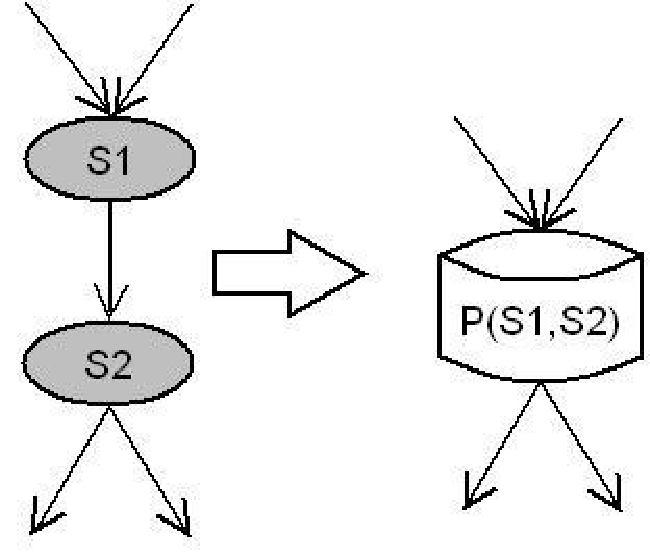
\includegraphics[width=12cm]{LanguageEngineering/Commands/Images/P}

\caption{A P-Reduction Pattern\label{fig:A-P-Reduction-Pattern}}

\end{center}
\end{figure}


\begin{lstlisting}
context Graph
  @Operation reduceP():Graph
    @Case self of
      // Find two nodes with a then-edge
      // between them, replace with a P
      // node...
      Graph(N->including(n1 = Statement())
             ->including(n2 = Statement()),
            E->including(e = Next())
        when e.source() = n1 and
             e.target() = n2) do
        self.reduce(P(e),Graph(Set{n1,n2},Set{e}))
      end
      // Otherwise, leave the receiver unchanged...
      else self
    end
  end
\end{lstlisting}A W pattern corresponds to a
while loop and occurs when a test node has a true outcome that is
a body statement whose next leads back to the test. The false outcome
leads to some root node for the rest of execution. The reduction involves
replacing the test and its body with a W node
and adding a new next edge from the W node
to the root. The reduction is shown in figure \ref{fig:A-W-Reduction-Pattern}.

%
\begin{figure}
\begin{center}

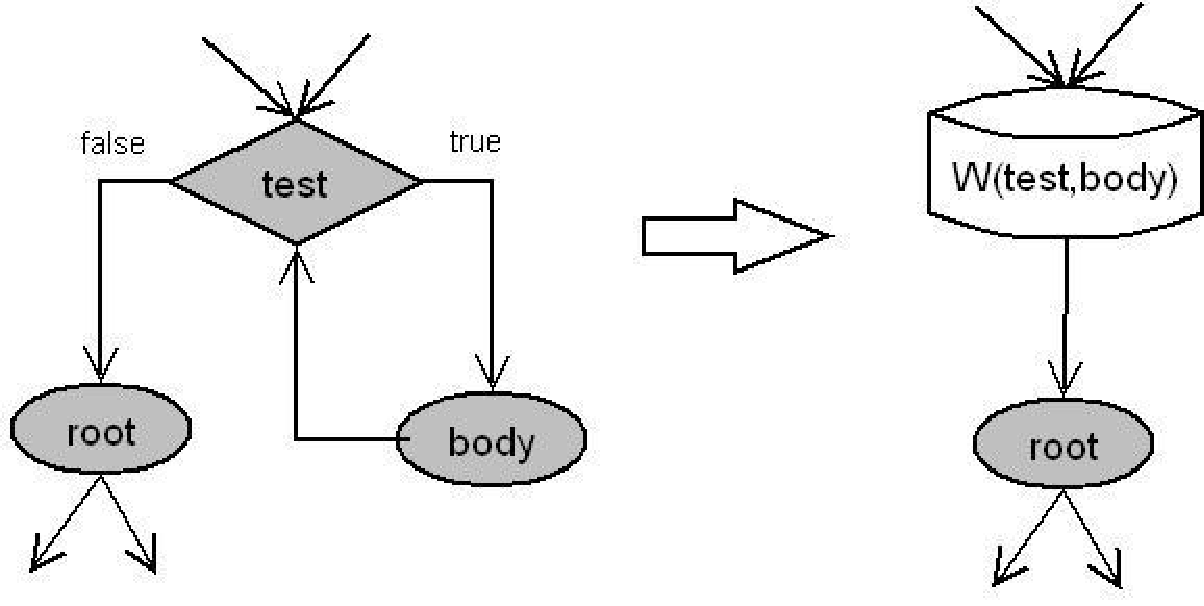
\includegraphics[width=12cm]{LanguageEngineering/Commands/Images/W}

\caption{A W-Reduction Pattern\label{fig:A-W-Reduction-Pattern}}

\end{center}
\end{figure}


\begin{lstlisting}
context Graph
  @Operation reduceW():Graph
    @Case self of
      // Find a test node and a statement that are linked
      // via a true outcome and a loop back to the test.
      // Replace them with a W node ...
      Graph(N->including(test = Guard())
             ->including(body = Statement())
             ->including(root),
            E->including(enter = True())
             ->including(loop = Next())
             ->including(exit = False())
        when enter.source() = test and
             enter.target() = body and
             exit.source() = test and
             exit.target() = root and
             loop.source() = body and
             loop.target() = test) do 
        let Wnode = W(test,body);
            H = Graph(Set{test,body),Set{enter,loop,exit}) then
            newEdge = Next(Wnode,root)
        in self.reduce(Wnode,H).addEdge(newEdge)
        end
      end
      // Otherwise, leave the receiver unchanged...
      else self
    end
  end
\end{lstlisting}A C pattern corresponds to an if statement and occurs when there is
a test node leading to two nodes both of which lead to a single root
node. This forms a diamond pattern with the test node at one end.
The test, then and else parts of the graph are removed and replaced
with a C node. The reduction is shown in figure \ref{fig:A-C-Reduction-Pattern}.

%
\begin{figure}
\begin{center}

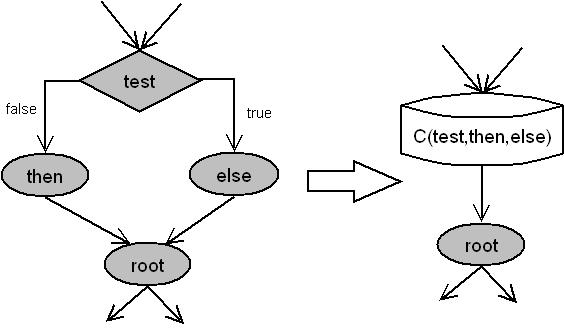
\includegraphics[width=12cm]{LanguageEngineering/Commands/Images/C}

\caption{A C-Reduction Pattern\label{fig:A-C-Reduction-Pattern}}

\end{center}
\end{figure}


\begin{lstlisting}
context Graph
  @Operation reduceC():Graph
    @Case self of
      Graph(N->including(test = Guard())
             ->including(thenNode)
             ->including(elseNode)
             ->including(root),
            E->including(trueEdge = True())
             ->including(falseEdge = False())
             ->including(endThen = Next())
             ->including(endElse = Next())
        when trueEdge.source() = test and
             trueEdge.target() = thenNode and
             falseEdge.source() = test and
             falseEdge.target() = elseNode and
             endThen.source() = thenNode and
             endThen.target() = root and
             endElse.source() = elseNode and
             endElse.target() = root) do
       let Cnode = C(trueEdge,falseEdge);
           H = Graph(Set{test,thenNode,elseNode},
                     Set(trueEdge,falseEdge,endThen,endElse}) then
           e = Next(Cnode,root)
       in self.reduce(Cnode,H).addEdge(e)
       end
     end
     else self
    end
  end
\end{lstlisting}Equality on graphs is defined in terms of the labels on the nodes
and edges. Two graphs G and H are equal when they have the same number
of nodes, when the respective sets of labels are equal, when the edges
of G correspond to the edges of 
H in terms of the source and target nodes and when the respective
sets of edge labels are equal. 

Graph reduction can involve more than one step. For example, certain
configurations of graph require a P reduction
to occur before a C reduction can occur. In
order to reduce a graph fully we continually perform a reduction until
no further reductions can take place:

\begin{lstlisting}
context Graph
  @Operation reduce():Graph
    let G = self.reduceP().reduceW().reduceC()
    in if G.equals(self)
       then G
       else G.reduce()
       end
    end
  end
\end{lstlisting}
